\section{Contexto}
En este diagrama nos permite ver los diferentes agentes y las interacciones entre los mismos a alto nivel, permitiendonos ademas saber que agente controla las acciones y quien las monitorea.Para este problema identificamos los siguientes agentes:

\begin{itemize}
\item Gerente
\item PM 
\item Administrador (Admin) 
\item Cliente 
\item Proveedor
\item Subsistema de Mail 
\end{itemize}

En el siguiente diagrama utilizaremos estos agentes para describir lo mencionado anteriormente.
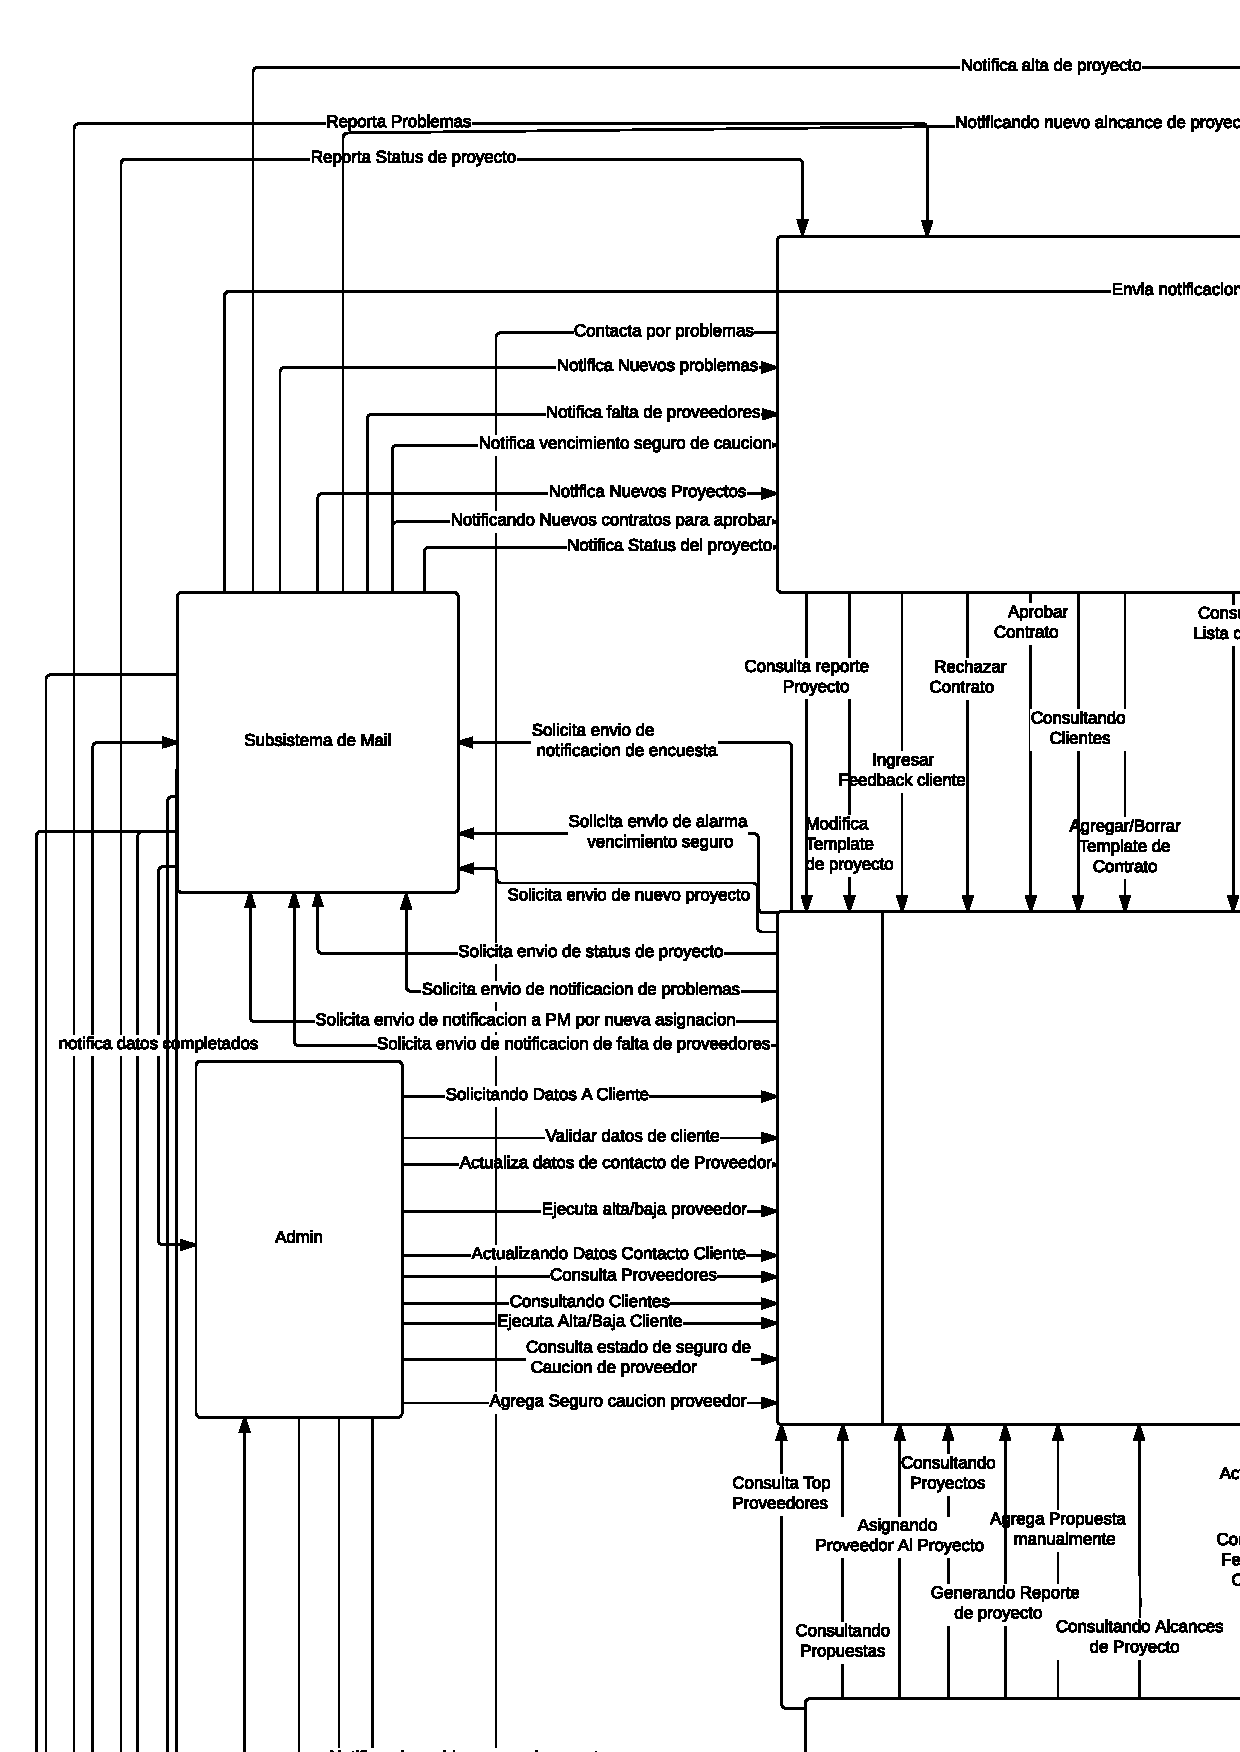
\includepdf[pages=-, offset=75 -75]{imagenes/contexto/contexto.pdf}
